There are a number of buttons in the Push Button area of \Cref{fig:generic_ui}. This section describes the usage of those buttons.

\subsection{RUN}

This button allows the user to run the simulation on the local machine. The window that pops up is as shown in \Cref{fig:run_button_popup}. There
are two input fields, and a button in the window. The typical user DOES NOT NEED TO MODIFY THE INFORMATION IN THE INPUT FIELDS. Advanced users can specify the locations of the following two directories here:

\begin{figure}[!htbp]
  \centering {
    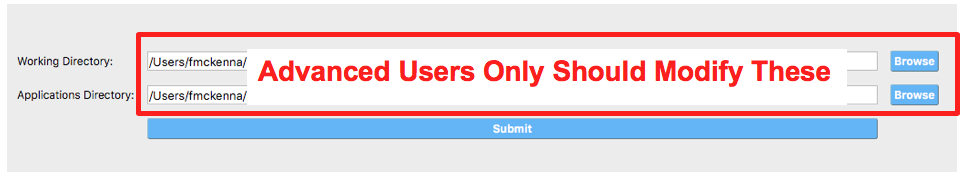
\includegraphics[width=0.8\textwidth]
    {usage/figures/runButton.png} }
  \caption{Pop-up window shown after clicking on the \texttt{Run} button}
  \label{fig:run_button_popup}
\end{figure}

\begin{itemize}
\item Working Dir Location: specifies where the \texttt{\getsoftwarename{}} application shall
create a \texttt{tmp.SimCenter} directory for temporary files that are used to perform the simulation. This directory is created after the \texttt{Submit} button is pressed. As discussed in \Cref{chap:troubleshooting}, when
the application creates this directory it copies the files needed to it (e.g., if you are using OpenSees input script, it
will copy that script to the \texttt{tmp.SimCenter} directory. ALL FILES IN
THE SCRIPT DIRECTORY AND ALL FILES IN SUBDIRECTORIES OF THAT DIRECTORY GET
COPIED SO DON’T PLACE THE OPENSEES SCRIPT IN HOME, DOWNLOADS, DOCUMENTS, etc….
\item Application Dir Location: The \texttt{\getsoftwarename{}} application searches for the workflow applications in this directory. Only edit its location if you are introducing your own applications or you want to build and modify the 
applications provided with the tool. 
\end{itemize}

Hitting the \texttt{Submit} button starts the simulation by running the various workflow applications. After the simulation finished, the pop-up window will close and the RES panel will be in focus. Please do not press the \texttt{Submit} button multiple times. It will not make the simulation run faster and might cause unexpected behavior.

\subsection{RUN at DesignSafe}
This button allows the user to package the input information, send it to DesignSafe and run the simulation remotely at the Stampede2 supercomputer. Simulation results will be stored in the user's DesignSafe jobs folder and can be retrieved with the \texttt{GET from DesignSafe} button. After clicking on the button, the window shown in \Cref{fig:remote_button} pops up. There are several input fields and a \texttt{Submit} button in the window. The typical user ONLY NEEDS TO EDIT THE TOP FOUR FIELDS. The purpose of the lower four fields is described below for advanced users. The following pieces of information are collected in the pop-up window:

\begin{figure}[!htbp]
  \centering {
    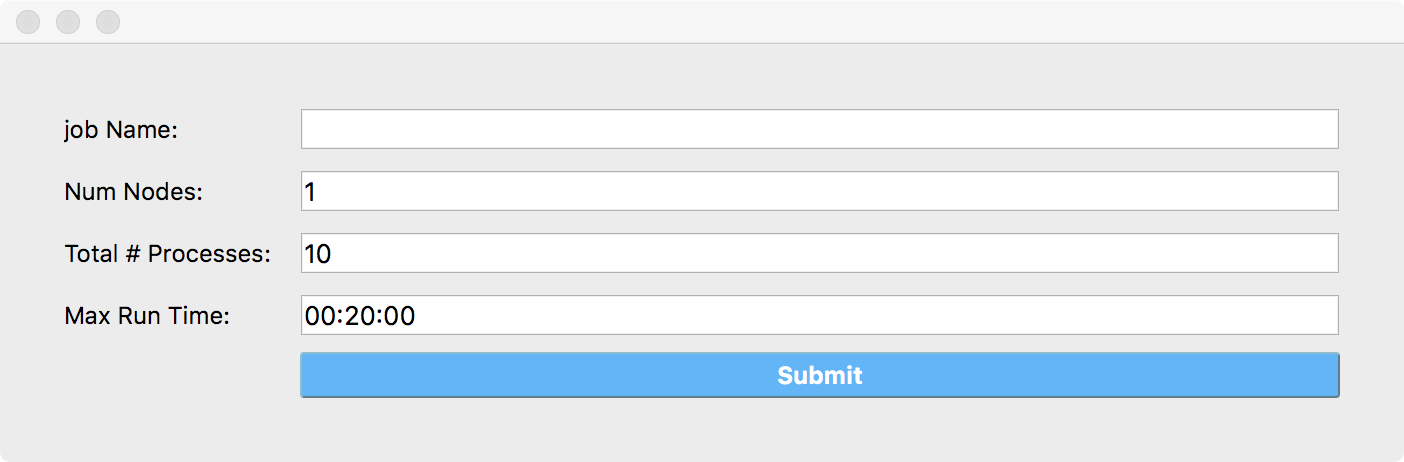
\includegraphics[width=0.8\textwidth]
    {usage/figures/remoteButton.png} }
  \caption{Pop-up window shown after clicking the \texttt{RUN at DesignSafe} button}
  \label{fig:remote_button}
\end{figure}

\begin{itemize}
\item Job Name: The name the user can use to identify the job in Get from DesignSafe.
\item Num Nodes: The number of compute nodes to use on Stampede2. Using the default App Name the job will run on Stampede2’s KNL Landing (KNL) 
compute nodes. Each node has 68 cores. The actual number of cores the
application will use on each of these nodes depends on the total
number of processes specified. As per the TACC webpage, for MPI tasks
it’s best not to specify more than 64-68 processes to run. Depending
on the numerical computations and amount of memory each uses, for large simulations you may wish to use more nodes and less processes to
avoid page faulting.
\item Total Number of Processes: Total number of MPI parallel processes the UQ engine is going to use.
\item Max Wall Time: Use HOURS:MIN:SEC format and be conservative. Your job is killed after the time limit is reached. On Stampede2 you have a max wall time of 24 hours.
\item App Name: Name of Agave app to run. Only modify if you know what you are doing.
\item Working Dir Location: specifies where the \texttt{\getsoftwarename{}} application shall
create a \texttt{tmp.SimCenter} directory for temporary files that are used to perform the simulation. This directory is created after the \texttt{Submit} button is pressed. As discussed in \Cref{chap:troubleshooting}, when
the application creates this directory it copies the files needed to it (e.g., if you are using OpenSees input script, it
will copy that script to the \texttt{tmp.SimCenter} directory. ALL FILES IN
THE SCRIPT DIRECTORY AND ALL FILES IN SUBDIRECTORIES OF THAT DIRECTORY GET
COPIED SO DON’T PLACE THE OPENSEES SCRIPT IN HOME, DOWNLOADS, DOCUMENTS, etc…. The Working Directory is removed after the job has been submitted successfully.
\item Local App Dir Location: The \texttt{\getsoftwarename{}} application searches for the workflow applications in this directory. Only edit its location if you are introducing your own applications or you want to build and modify the 
applications provided with the tool. 
\item Remote App Dir Location: Remote directory on Stampede2 where applications needed by the workflow reside. Only modify if you know what you are doing.

\end{itemize}

\subsection{GET from DesignSafe}
Allows you to obtain your list of jobs from DesignSafe and select from that list a job to update status of, download or delete.

\subsection{Exit}
Click this button to exit the application.